This section provides a commentary of the implementation work of the framework.
We will also take a closer look at the performance of the finished framework and where improvements can be made in the future.
To allow our work to be put into perspective, we will also compare the framework with the Aruco framework.
For that we implemented a basic application that implements the functionality of Imagine.

\section{Implementation}
\label{implementation}

Here we will take a look at the process of implementing Imagine.
First we will discuss difficulties and hardships endured during actual coding.
Then we will take a closer look at the performance of the completed framework.

\subsection{Encountered Difficulties}

% Sparse help
The first major difficulty we encountered upon beginning the implementation was the user generated documentation of the Java OpenCV for Android framework in the form of questions and answers or tutorials.
The probable cause for this is most likely due to the fact that OpenCV was originally written for desktop applications using C++.
That means that there are two major differences between the more widely used and documented version of the framework compared to the version used for this project.
The first is that one of the goals of our work was to write a Java framework, thus encouraging that we use the Java wrapper for OpenCV – therefore making the majority of C++ resources moot and hard to use.
The second difference is due to the fact that our framework's platform was to be Android, for which a few small differences existed compared to the normal use of OpenCV – such as the use of OpenCV via the elegant solution of a separate application, the OpenCV manager.
These two differences seem to have been sufficient in decreasing the usage of the Java port of OpenCV enough that documentation and accessible tutorials and examples proved to be far in between.
This forced development to rely all too often on examples written for other platforms and programming languages.
Luckily however the framework syntax is consistent, although the used data types are not always transferable.
Thus such translation work was possible but difficult.

% Lacking documentation
But not only unofficial documentation is lacking: official documentation in the form of documentation for the application programming interface and official tutorials are, for all intents, almost non existent at the time of this paper.
Comparably to the lacking user generated documentation, this can be mitigated by using material intended for C++.
C++ documentation is also all there is for the Javadoc used within the IDE.
It is not easy working in Java with C++ code as Javadoc, with further text mostly not relevant to the problems encountered when coding with it.

% Problems with stupid mat
While we're on the topic of the C++ base of OpenCV, allow us to criticize the single most frustrating aspect of using OpenCV: the matrix object data type, short mat.
Mats are used within OpenCV as a one-size-fits-all solution for any data ranging from vector points that represent polygons to multi-channel images in various more or less used formats.
While it was still easy to recognize the RGBA format\footnote{RGBA stands for, respectively: red, green, blue, alpha. This depicts the order and type of channels for an image.} that the framework receives the camera image in, using the correct conversions and the correct mat subtypes in the principle work thread within Imagine proved to be very frustrating.
First we encountered difficulties with the conversion of different image formats to other formats, an operation that costs a good bit of processing power and time.
Thankfully, we were able to work around any conversions by parallel usage of multiple mats whose results are used on one another to retain a higher overall speed.

Then another difficulty emerged while using the OpenCV function to calculate polygons for detected contours within an image.
The method for these polygons returns these in a special mat subtype that is specialized for floating point numbers.
However, the methods we then required to work with these polygons required the polygons in a normal mat, thus forcing us to convert from one type of mat to another.
Again this problem could largely be mitigated by converting as little as possible, although the base conversion proved to be one of the smaller problems in the overall context of speed within the Imagine worker threads.
Furthermore, there exist no methods for determining the type and allocation of channels within a mat.
While not being able to check for these properties forced a clean usage of the data class within Imagine and thus probably increased speed somewhat, such methods are crucial for learning the correct usage of mat and certainty of stored data type.
Writing and reading data with mats is also something that requires faith, as no checks for sanity can be performed on the data.
For example, the method for reading a single coordinate returns a double array – always, even when using the mat for binary images (in which case a boolean would suffice), luminance images (possibly a short data type), or as an integer matrix (integers).
The returned value then has to be cast to the (hopefully) correct data type – and if we made a mistake somewhere along the line and the mat doesn't contain the data we expect it to contain, we have no tools that would help us catch that mistake.
We therefore kindly suggest that OpenCV for Android make use of the Java generics mechanism, as we believe that would start to reduce the confusion surrounding mats.

% Problems debugging
A further difficulty proved to be the debugging of errors while programming the worker threads within Imagine.
This came from the fact that OpenCV runs in C++ even on Android and tracing errors to their source thus proved difficult.
Often only careful consideration of error messages and stack traces in the depths of the Android log allowed any progress to be made in tracing a bug, although mostly trial and error proved to be the primary method of correcting these errors.
Problems debugging errors were also due to the paradigm differences in error handling between how Java in general does it (using so-called exceptions) and C++ does it (using integers as error codes).
OpenCV for Android does not cast the numeric error codes into equivalent Java exceptions, instead leaving them as-is.
Furthermore, the numerical error codes proved to be very generic in their implications.
An example of this can be found with the error code we mostly fought with, which was 215.
That numerical error can (and does!) mean anything from incorrect mat sizes to incorrect number of channels.
A quick search also showed that the very same code is also used to signal unimplemented methods within OpenCV itself.

% Paradigm problems
While on the topic of paradigm differences: another difficulty we encountered with OpenCV for Android was the difference in coding styles.
With this we mean for example that the result of a method was not returned, but instead called by reference\footnote{This stems from the way C++ usually does error handling by returning numerical error codes. The result is written into a referenced data class, freeing the return call for passing back numerically coded error or success messages.}.
Due to the existence of exceptions, this is usually done differently when using Java.
While generally more of a nuisance than a source of error, it would be helpful if the wrapper took care of the paradigm shift between Java and the C++ interface, thus freeing developers from having to work with two paradigms in parallel.

% General
Generally speaking, OpenCV for Android proved usable for this work, but with some difficulty, as can be seen by the lengthy dissection here.
OpenGL ES proved to relatively trivial to use, notably because of the wealthy online resources in the form of extensive documentation and multiple tutorials.
The only bigger difficulties encountered while working with OpenGL ES were using multidimensional math for the matrix operations and how to get the renderer to render to a transparent layer.

\subsection{Performance}
\label{performance}

Here, we will take a brief look at the general performance of the Imagine framework.
All numbers that will be given are approximations only, as we did not statistically analyze them.
For a more in depth look of Imagine's performance, further work can be done as necessary.

\subsubsection{Frames per Second}

To give the following numbers a frame of reference, here some numbers concerning the general speed of the Android platform, and the OpenGL ES and OpenCV utilization on it.

OpenCV captures the preview frame of the camera from Android for the base frame from which all processing originates.
This means that the speed at which it does this is the first important reference for all further values.
The speed of this operation proves to be the first limiting factor: due to how Android camera capture works, the preview only offers 15 frames per second.
This was measured by simply showing the image as received through OpenCV, meaning that there was no overhead work being done.
This has some strong implications for the Imagine framework: however much the work done can be optimized, it will never be capable of running faster than that.
As humans only begin to see a smooth video upwards of approximately 20 frames per second – for perfectly smooth video however at least 60 frames per second – this places Imagine already outside the range of smooth output.

Android itself renders the interface at 60 frames per second\footnote{As of Android 4.1.}.
OpenGL ES also easily achieves 60 frames per second, although it is to note that the graphic pipeline has the advantage of serious hardware acceleration.
Of course the speed at which OpenGL ES will render a scene for the Imagine framework is highly dependent on the complexity of the models, although that should not be a limiting factor for some time yet.

The comparison of these two limiting factors shows that Imagine is mainly performance dependent on the OpenCV for Android framework.
Newer versions of it should theoretically be able to increase the speed up to the framerate of the camera preview.
To achieve even higher speeds, the speed at which Android fetches the camera preview must be increased, which could happen with newer devices and or newer version of Android.
All of these possible speed increases however lie outside of the influence of the Imagine framework.

\begin{figure}[H]
	\centering
	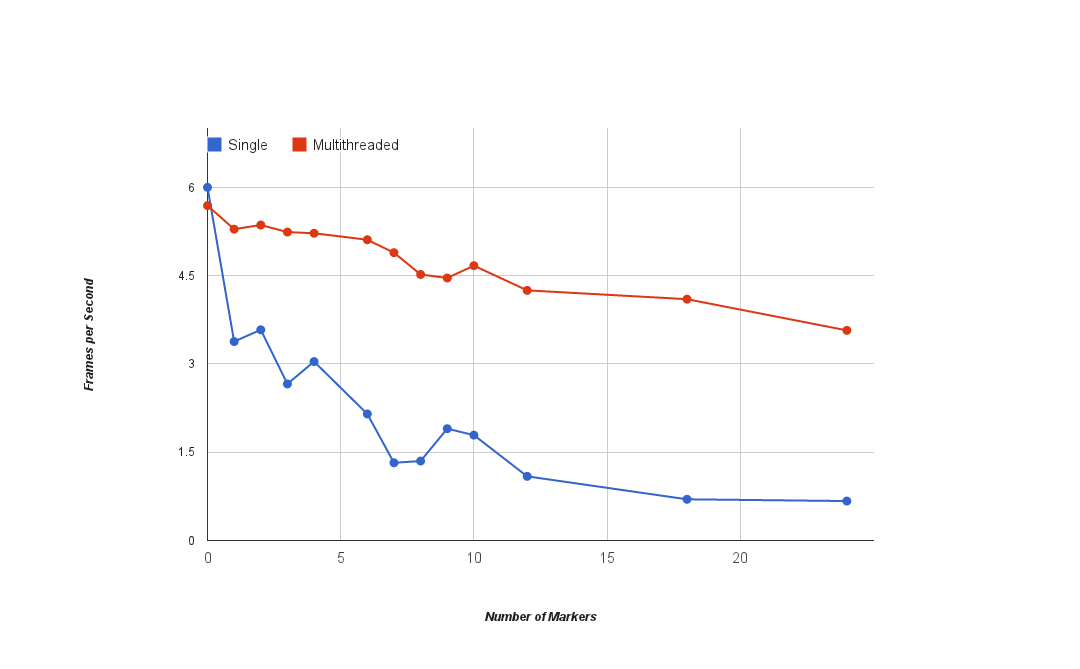
\includegraphics[width=16cm]{img/performance_chart.png}
	\caption[Imagine Performance Chart.]{This chart shows the performance in frames per second of Imagine, working both as a single pipeline and with multithreading.}
	\label{fig:performance_chart}
\end{figure}

For the speed of the Imagine framework, a general understanding of the algorithm that detects markers is required – as can be found in section \ref{detection_workflow}.
Imagine idles at up to \textbf{seven frames per second}, meaning that this is the best case performance under ideal circumstances with no markers present.
When markers are present and detected, performance takes a hard dip.
This and the difference multithreading makes can be seen in figure \ref{fig:performance_chart}.

\subsubsection{Speed of Operations in Detector}

The first performance sensitive operation is the \textbf{conversion of the input image into a binary image}.
The default method with a static threshold takes around 8 ms.
It is significantly faster than adaptive thresholding with 88 ms.
However it does not work reliably in low contrast images or in high dynamic ranges within an image.

Next is the \textbf{operation that finds all contours from the binary image}.
This operation is a vital part of the algorithm and can not easily be exchanged for some other operation.
The cost of finding contours varies strongly on the binary image, but generally takes around 22 ms.

Now Imagine has to \textbf{process each contour separately}, as each could be a marker.
This step is where most of the performance is siphoned from.
In total these operations take around 100 ms, with a high variance for the number of markers.

For each found contour, we \textbf{calculate the polynomial approximation} and use it to filter out any polygons that aren't convex and don't have 4 corners.
This step takes about 3 ms.
Imagine then calculates the perspective transform and applies it to \textbf{dewarp the texture} of the marker candidate to allow sampling.
Using the RGBA input mat, OpenCV does this step in 12 ms.
Originally however we require a grayscale image at this point; however it turns out that OpenCV has no hardware acceleration for dewarping grayscale mats on a Tegra CPU, such as the developer machine has.
Using the grayscale image would impose a more hefty performance cost.

If the contour is still a valid candidate at this point, Imagine tries to \textbf{detect a marker} from it and the dewarped texture.
This method takes anywhere from 5 ms to 30 ms, depending on whether the candidate is valid in terms of sampling its properties from the texture (meaning valid border, orientation, and identification marks).
If a marker is rotated, then the correction of the identification pattern takes additional time, as rotating matrices is computationally expensive.

Now only one step remains for a complete marker detection: \textbf{calculating the perspective transformations}.
This is done for all detected markers, but luckily is relatively fast compared to other operations.
OpenCV takes 2 ms to calculate the data for every marker.

\section{Features and Capabilities}

In this section, we will take a look at the implemented features of Imagine.
This includes basic features that are required for basic usability and capabilities for debugging various algorithm stages.

\subsection{Debugging Capabilities}

Imagine offers some easy options for selective debugging beyond the log output on Android.
Specifically for debugging the visual pipeline we implemented some options so that pinpointing an error is comparatively easy.
Setting debugging up is done via flags and should only be done before calling the onCreate method.

The first option we offer is to \textit{activate a more verbose logging mode}, where Imagine logs quite a bit more information concerning possible errors – for example, the status of the hamming decoding upon marker detection.
On par with that one can also \textit{activate frame per frame time logging}, where Imagine will log the time each detection and rendering step takes.

Going into the visual debugging it is important to note that marker detection is partially suspended.
In any case Imagine deactivates multithreading to enable the output to be shown – as seen in section \ref{performance}, this decreases performance quite a bit.
Once in visual debugging mode, three main aspects can be shown.
The first option that can be activated \textit{shows the binary picture}.
This can be used to check whether the chosen binarization method is working correctly.

Another output that can be chosen is to let Imagine \textit{draw the detected contours}.
This option can be used to detect errors within the contour detection that arise from the method used to binarize the image.

\begin{figure}
	\centering
	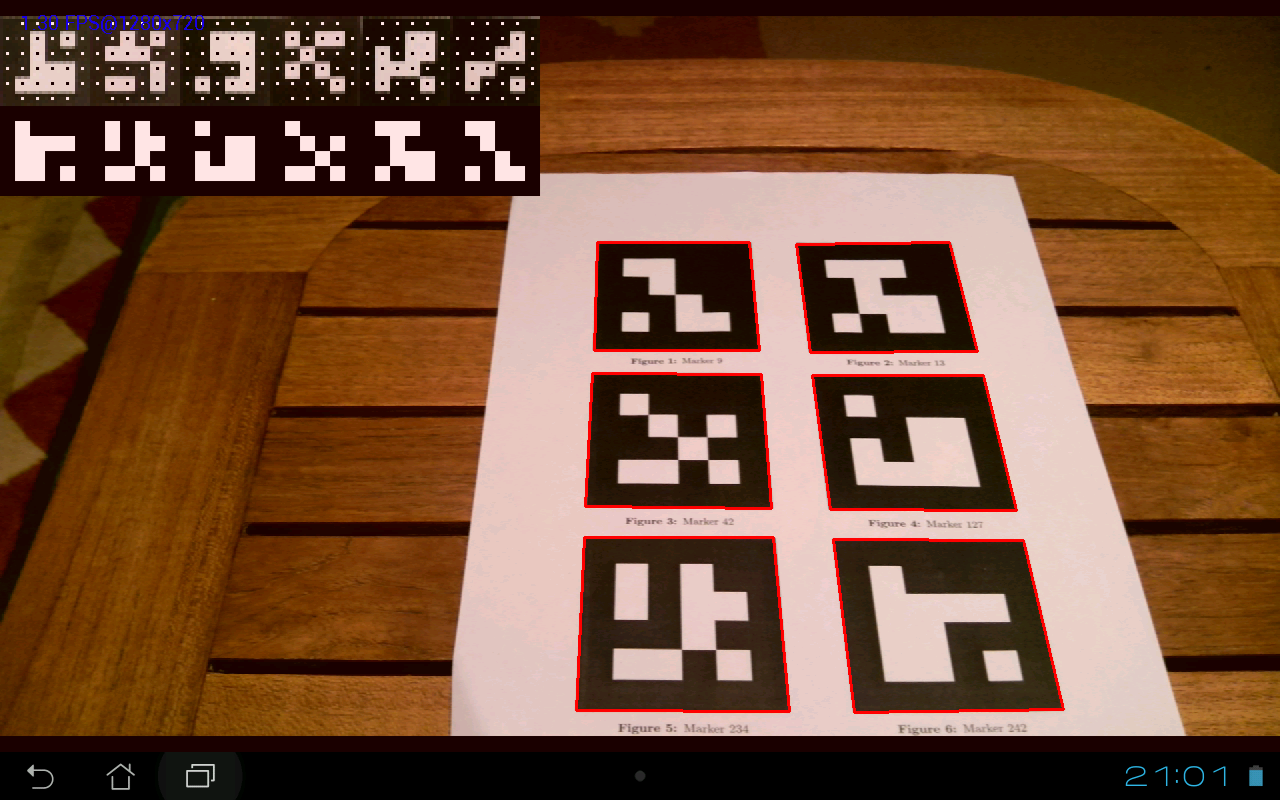
\includegraphics[width=10cm]{img/debugging_view.png}
	\caption[Debugging View]{A screenshot of how the three more relevant debugging views can look. Shown are the polygonal rendering (perspective red squares around markers), the marker texture with the sampling points, and the correctly rotated processed marker pattern.}
	\label{fig:debugging_view}
\end{figure}

The following visual debugging methods are the more helpful ones.
Figure \ref{fig:debugging_view} shows how the polygonal rendering, the texture sampling of markers, and the detected identification pattern are shown.

Of these, the option to display the polygons of detected markers is best used to check that Imagine sees a marker.
Here, Imagine draws the perspective bounding box of all marker candidates that have been detected.
To check whether Imagine correctly samples a marker candidate, both the option to draw the marker textures and the marker identification patterns can be used.
Drawing marker textures can verify that Imagine has correctly dewarped a texture and show how warped the marker surface was.
This can be seen when the dewarped marker texture is not perfectly aligned with the square sampling.
The marker identifications can be used in conjunction with the option to draw the sampling onto the marker textures to check whether Imagine is correctly sampling the pattern of candidate markers.

All of these debugging capabilities arose out of the step-by-step development process.
Once we realized how useful such functions were, we decided to keep them accessible from the outside.
Thus we made sure that they work relatively well and can be activated easily\footnote{This is realized by the methods in MainInterface for setting and removing debugging flags.}.

\subsection{Features}

Of the features listed in section \ref{scope_limit}, the following are accessible and usable.
Debug messaging is possible beyond the functionality already offered by Android, most notably a unified logging mechanism and timing functions.
Managing so-called trackables is possible, including the on-the-fly adding, removing, and exchanging of marker-object associations.
Reading the pure 3D transformation data is also possible via a listener, bypassing the graphical part of Imagine.
Manual configuration is somewhat possible, as many values can be changed to accomondate special use cases.
It is however easily possible to configure debugging views to display relevant information and to enable extensive debugging output.
Multithreading is also implemented and beneficial, as seen in section \ref{performance}.
If required or when debugging views are to be used, a single thread pipeline can also be used.

Therefore we conclude that our framework covers the basics in functionality, although a multitude of improvements can be made.
These improvements are listed in section \ref{improvements}.

\section{Application}

To enable rapid testing and experimenting, we implemented a basic application for evaluating our framework.
It consists of two activities: one for setting parameters and control values and one for actually running the framework.

Figure \ref{fig:debugging_view} is a screenshot of the application running the framework activity with debugging values activated.

TAMINO TODO: TODO AND MORE!

\section{Comparison to similar Apps}

In this section, we will compare Imagine to two other marker-based augmented reality frameworks for Android.
Both are open source projects and can be used freely in personal projects.
Table \ref{comp} lists the main differences.

\begin{table}[H]
	\centering
	\begin{tabulary}{\textwidth}{J | J | J | J}
	\textbf{Framework} & \textbf{FPS} & \textbf{Number of markers} & \textbf{Maximum parallel markers} \\
	\hline
	Imagine & ~5 & 256 & 256 \\
	\hline
	Aruco & ~4 & 1024 & unknown \\
	\hline
	DroidAR & unknown & 4096 & 5 \\
	\end{tabulary}
	\caption[Performance Comparison]{Short table of feature comparison of Imagine, Aruco, and DroidAR.}
	\label{comp}
\end{table}

\subsection{Aruco}

Aruco \cite{aruco} is a minimal library for Augmented Reality applications based on OpenCV.
Primarily, it is intended for desktop C++ applications, although an Android port and web-based Javascript port exist.
For the purpose of comparing it to our own framework, we will base the comparison on the Javascript port \cite{jsaruco} running on the same developer machine.

\begin{figure}[H]
	\centering
	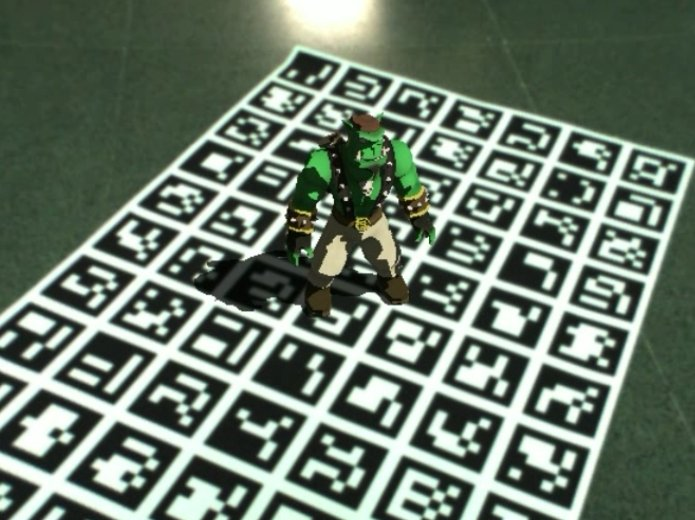
\includegraphics[width=8cm]{img/aruco.png}
	\caption[Aruco]{Screenshot of a basic Aruco application.}
	\label{fig:aruco}
\end{figure}

The main features of Aruco are simple usage, 1024 markers that can be identified, and the support of so-called AR boards\footnote{Markers composed of several markers for higher reliability.}.
The marker detection algorithm used by Aruco is the basis for our own work and thus works similarly.
The main differences in implementation are that Aruco does sub pixel accuracy and a higher number of markers.
These are advantages of Aruco over Imagine.

The Javascript port runs at around four frames per second in a mobile web browser.
This is a low difference compared to Imagine, although our framework runs natively.
We believe this due to the fact that while Aruco is based on OpenCV, the Javascript port can not use the library, and thus re-implements the required features.
That removes any overhead caused by unused features and allows a completely native environment for data objects, without any significant conversions having to be done, which were one bottleneck in Imagine.
Nonetheless Imagine is a small step faster.

\subsection{DroidAR}

DroidAR\cite{droidar} is another framework for Android that allows, among other Augmented Reality features, marker-based tracking.
Due to difficulties using the framework on the developer's machine, no performance comparison could be made.
DroidAR could not be tested solely without any other features without writing an application for that, which is beyond the scope of this comparison.

\begin{figure}[H]
	\centering
	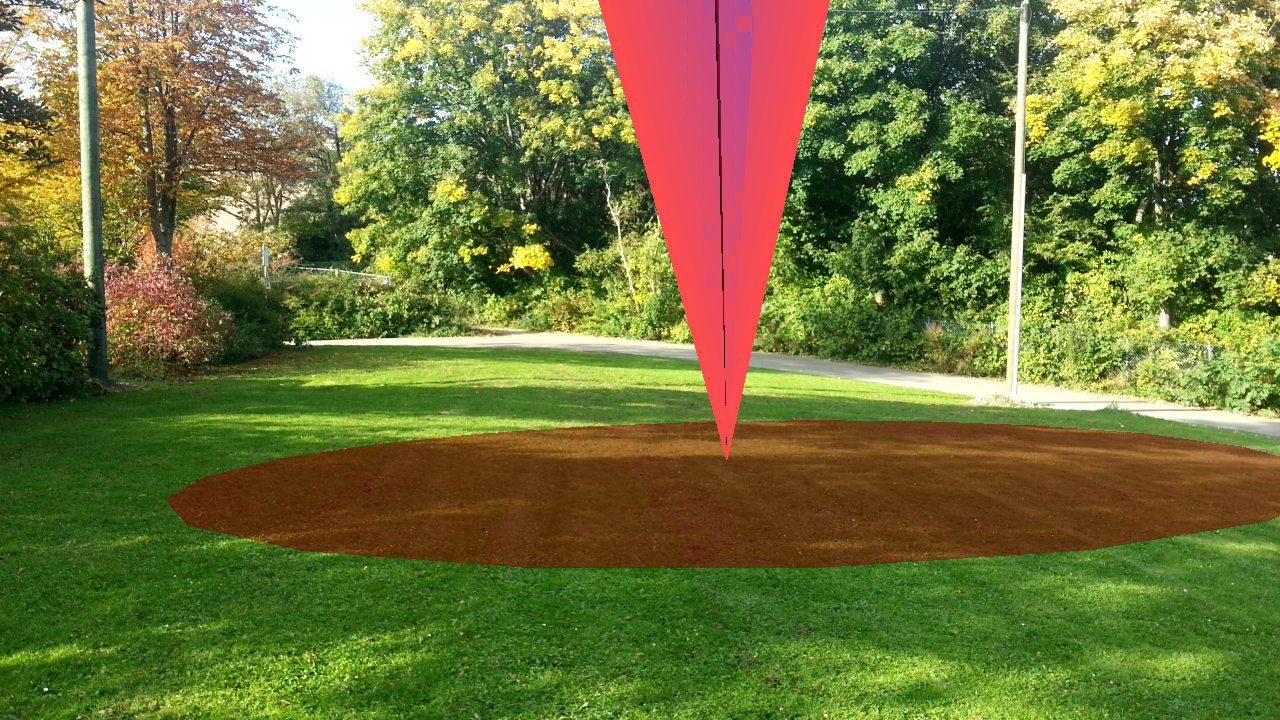
\includegraphics[width=10cm]{img/droidar.png}
	\caption[DroidAR]{Screenshot of a basic DroidAR application.}
	\label{fig:droidar}
\end{figure}

Feature wise a few things are different compared to Imagine, although some interesting parallels also exist.
Most notably, DroidAR uses threads for the detection of markers and also utilizes OpenCV for Android.
The detection method is also similar to both Aruco and Imagine.
However, the actual detection is done with native C++ code.
DroidAR can differentiate 4096 markers, although only 5 can be detected at once, probably for performance reasons.
Imagine can detect more than 5 markers in parallel, DroidAR however has a faster implementation.
